% requires CTAN package tikzposter, xelatex, and Calibri font
\documentclass[a1paper,25pt]{tikzposter}% use 20pt for more text
\usetheme{Simple}

%%% VZG STYLE %%%%%%%%%%%%%%%%%%%%%%%%%%%%%%%%%%%%%%%%%%%%%%%%%%%%%%%%%%%%%%%%%%

\definecolor{GBV}{RGB}{89,124,199}
\definecolor{GBVDark}{RGB}{0,51,153}

\definecolorstyle{gbvColorStyle}{
  \definecolor{noteColor}{HTML}{FCE565}%FCF0AD}
}{
  % background colors
  \colorlet{backgroundcolor}{white}
  \colorlet{framecolor}{white}
  % title colors
  \colorlet{titlefgcolor}{white}
  \colorlet{titlebgcolor}{GBV}
  % block colors
  \colorlet{blocktitlebgcolor}{GBV}
  \colorlet{blocktitlefgcolor}{GBVDark}
  \colorlet{blockbodybgcolor}{white}
  \colorlet{blockbodyfgcolor}{black}
  % innerblock colors
  \colorlet{innerblocktitlebgcolor}{white}
  \colorlet{innerblocktitlefgcolor}{black}
  \colorlet{innerblockbodybgcolor}{white}
  \colorlet{innerblockbodyfgcolor}{black}
  % note colors
  \colorlet{notefgcolor}{black}
  \colorlet{notebgcolor}{noteColor!70!white}
  \colorlet{notefrcolor}{noteColor}
}

\makeatletter
\TP@showlatexaffectionfalse

\newcommand{\email}[1]{\def\@email{#1}}
\newcommand{\doi}[1]{\def\@doi{#1}}
\newcommand{\license}[1]{\def\@license{#1}}
\newcommand{\about}[1]{\def\@about{#1}}
\newcommand\titlelogoleft[2][]{\def\@titlelogoleft{\includegraphics[#1]{#2}}}
\newcommand\titlelogoright[2][]{\def\@titlelogoright{\includegraphics[#1]{#2}}}

\definetitlestyle{FilledWithLogo}{
    width=\paperwidth, roundedcorners=0, linewidth=0pt, innersep=1.5cm,
    titletotopverticalspace=0mm, titletoblockverticalspace=20mm,
}{
   \draw[draw=none, fill=titlebgcolor]%
   (\titleposleft,\titleposbottom) rectangle (\titleposright,\titlepostop); % 
   \ifdefined\@titlelogoleft\node at (\titleposleft,\titleposbottom) [anchor=south west] {
       \@titlelogoleft};
   \fi%
   \ifdefined\@titlelogoright\node at (\titleposright,\titleposbottom) [anchor=south east] {
       \@titlelogoright};
   \fi%
}
\settitle{ \centering \vbox{
    \centering
    \color{titlefgcolor} {\bfseries \Huge \resizebox{0.95\linewidth}{!}{\@title} \par}
    \vspace*{1em}
    {\LARGE \@author\\ \Large \texttt{\@email} \\[0.8em] \@institute}
  }
}

% show DOI, date, license, and about
\let\old@maketitle\maketitle
\renewcommand{\maketitle}{
    \old@maketitle
\begin{pgfonlayer}{backgroundlayer}
  \clip (bottomleft) rectangle (topright);
  \ifdefined\@about
    \node[inner sep=4pt, anchor=south west, draw=none]
      at (-0.5\textwidth+7pt, -0.5\textheight+7pt){\@about};
  \fi
  \node[inner sep=4pt, anchor=south, draw=none]
    at (7pt, -0.5\textheight+7pt){
      \ifdefined\@doi 
        \href{https://doi.org/\@doi}{DOI \@doi}
      \fi    
      \ifdefined\@date 
        (\@date)
      \fi    
  };
  \ifdefined\@license
    \node[inner sep=4pt, anchor=south east, draw=none]
      at (0.5\textwidth-7pt, -0.5\textheight+7pt){\@license};
  \fi
\end{pgfonlayer}
}
\makeatother

\usecolorstyle{gbvColorStyle}
\usetitlestyle{FilledWithLogo}
\useblockstyle{Minimal}
\useinnerblockstyle{Table}
\usenotestyle{Sticky}

\usepackage{fontspec}
\setmainfont{Calibri}
\renewcommand*\familydefault{\sfdefault}

\usepackage[colorlinks=true,citecolor=GBVDark,urlcolor=GBVDark,linkcolor=GBVDark]{hyperref}

%%% END OF VZG STYLE %%%%%%%%%%%%%%%%%%%%%%%%%%%%%%%%%%%%%%%%%%%%%%%%%%%%%%%%%%%

\usepackage{adjustbox}
\usepackage{nicefrac}

% coli-conc / VZG logo
\titlelogoleft[height=40mm]{coli-conc-logo}
\titlelogoright[height=30mm]{vzglogo}

\usetikzlibrary{shapes.geometric}

% references
\usepackage{lipsum}
\usepackage[backend=bibtex]{biblatex}
\addbibresource{bibliography.bib}
\renewcommand*{\bibfont}{\footnotesize}

% metadata
\title{Terminology Registries and Services}
\author{Jakob Vo\ss, Jana Maria Agne, Uma Balakrishnan, Morsheda Akter}
\date{2016-11-28}
\email{\{voss,agne,balakrishnan,akter\}@gbv.de}
\institute{Verbundzentrale des GBV (VZG), G\"ottingen}
\doi{10.5281/zenodo.166717}
\license{
\includegraphics[width=30mm]{cc-by}}
\about{
  coli-conc funded by 
\includegraphics[height=1em]{dfg-logo}
}

% bugfix to marry tikzposter & hyperref
\def\HyperFirstAtBeginDocument#1{#1}

% poster content
\begin{document}
\maketitle

\begin{columns}
\column{.5}
\block{Terminologies}{

  Terminologies, also known as Knowledge Organization Systems or vocabularies,
    help to agree on common concepts in data. Many types of terminologies exist
    \cite{Voss2016a} such as simple concept lists (e.g. Dublin Core Element
    Set), authority files (ORCID), classification systems (DDC), Thesauri
    (EuroVoc), and ontologies (Gene Ontology).

}
\note[angle=-35,width=115mm,targetoffsety=-3mm,rotate=2]
    {\url{http://bartoc.org/} lists $>$ 2.500 terminologies}


% Where to find and access terminologies?
\column{.5}
\block{Terminology Registries}{

 Terminology registries \cite{Golub2014} can broadly be classified into

  \begin{tikzfigure}
    \begin{tabular}{ll}
      \textbf{Registries}   & list and describe terminologies\\
      \textbf{Repositories} & contain full terminologies\\
      \textbf{Services}     & provide access to terminologies via an API\\
    \end{tabular}
  \end{tikzfigure}
  \vspace*{0.4em}
  \textit{Examples:} BARTOC \cite{Ledl2016,Voss2016b},
  GFBio Terminology Service \cite{Karam2016}
}

\note[angle=-85,targetoffsety=15mm,width=220mm,rotate=-2]
  {\url{http://bartoc.org/en/terminology-registries} 
    lists 74 registries, repositories, and services}

\end{columns}

\block{Terminology Services}{

  Query capabilities and APIs differ largely among Terminology Services.
  We developed the JSKOS format for Knowledge Organization Systems \cite{JSKOS}
  based on SKOS and JSON-LD to unify access to terminologies and registries
  especially for web applications \cite{Ledl2016,Voss2016b}.
%          \url{https://gbv.github.io/jskos/}

  \hspace{3mm}

  \begin{minipage}[t]{0.4\linewidth}

    Most APIs are "RESTful" web service: applications can access terminology
      data via HTTP on any platform and language.  Typical content types
      include SKOS/RDF and JSON based formats such as JSKOS. Queries are either
      responded from a local database or via wrapping an external web service.

  \end{minipage}%
  \begin{adjustbox}{valign=t}
    \begin{minipage}[t]{0.6\linewidth}
      \begin{tikzfigure}
        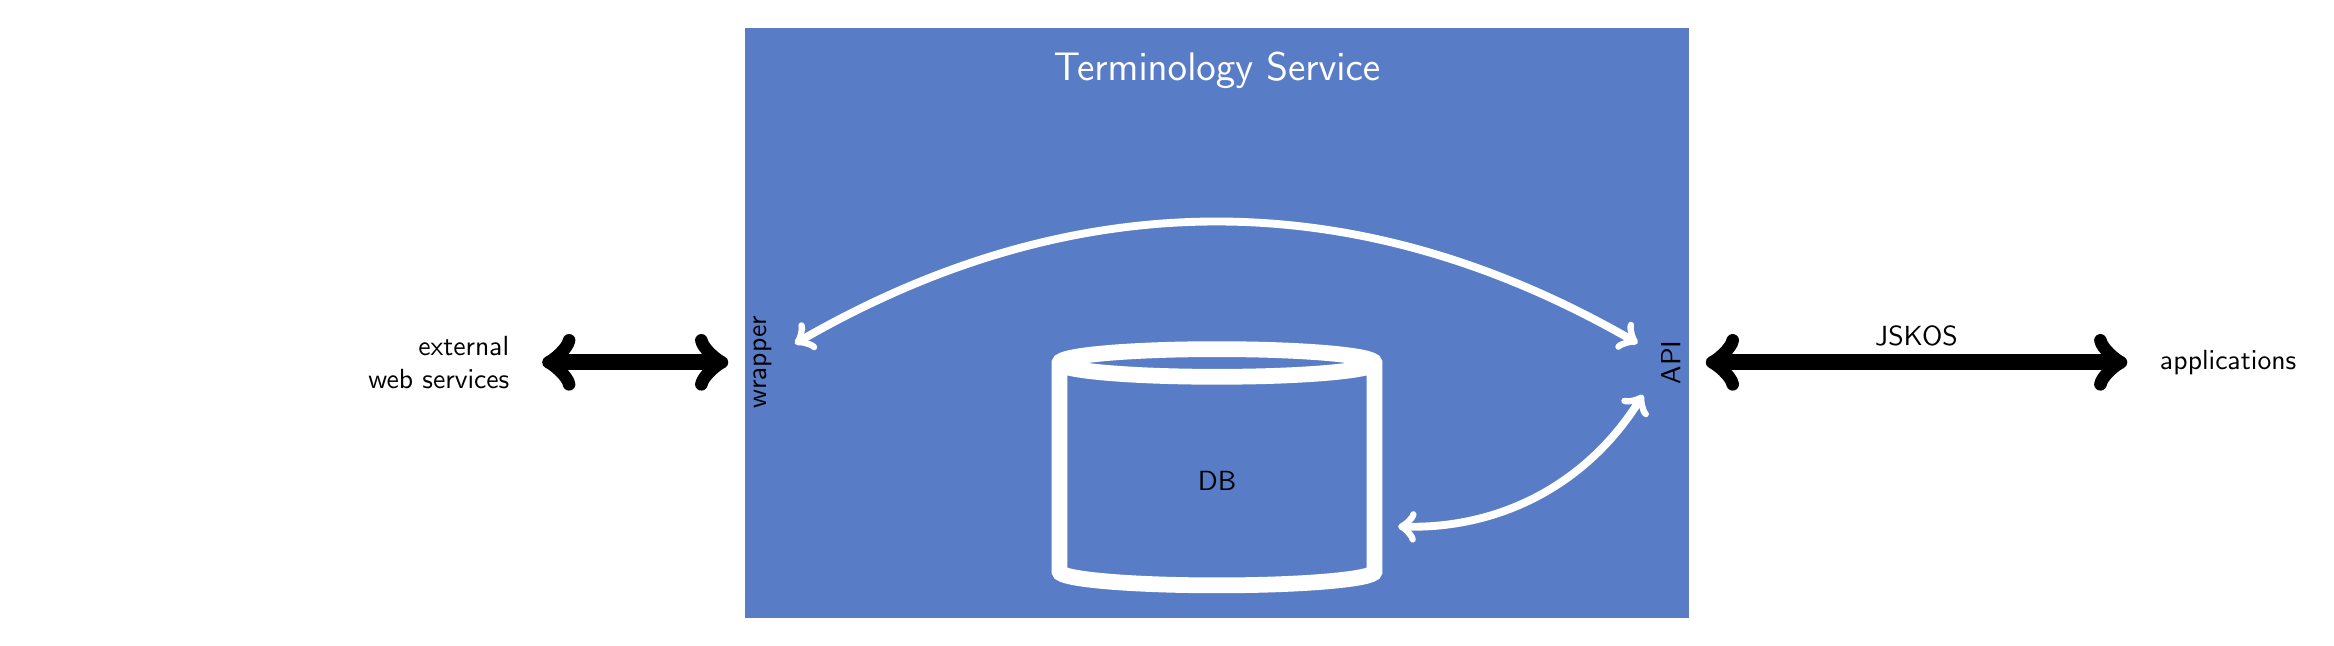
\begin{tikzpicture}
            \node[minimum width=12cm,minimum height=75mm,fill=GBV] (service) at (0,0) {};
            %\node[text width=50mm,align=center] at (-3mm,15mm) {\Large Terminology\\Service};
            \node[anchor=north,yshift=-2mm,color=white] at (service.north) {\Large Terminology Service};

            \node[draw=white,line width=2mm,cylinder,
                  shape aspect=1.5,rotate=90,minimum width=40mm,minimum height=30mm,
                  ] (db) at (0,-20mm) {};
            \node at (0,-20mm) {DB};

            \node[fill=GBV,rotate=90,anchor=north,xshift=-5mm] (wrapper) at (service.west) {wrapper};
            \node[fill=GBV,rotate=90,anchor=south,xshift=-5mm,minimum width=30mm] (api) at (service.east) {API};

            \begin{scope}[every path/.append style={<->,shorten >=2mm,shorten <=2mm}]
              \draw[line width=2mm] (wrapper) to +(-30mm,0) 
                  node[anchor=east,text width=60mm,align=right] {external\\ web services};
              \draw[line width=2mm]  (api) to 
                node[anchor=south] {JSKOS} +(60mm,0) node[anchor=west] {applications};

              \draw[draw=white,line width=1mm,bend right] (db) to (api);
              \draw[draw=white,line width=1mm,bend left] (wrapper) to (api);
            \end{scope}
        \end{tikzpicture}
      \end{tikzfigure}
    \end{minipage}
  \end{adjustbox}

}

%TODO: https://terminology.gbv.de (!)

%\note[angle=-50,rotate=5,width=185mm]
%  {See GFBio Terminology Service \cite{Karam2016} at Poster~2 by Müller-Birn \& Karam for an example!}


%Additional possible service features:
%simple search, hierarchies, mappings, reasoning


\block{Survey of registries, repositories and services listed in BARTOC}{
  \begin{minipage}[t]{0.38\linewidth}

    \begin{tikzfigure}
    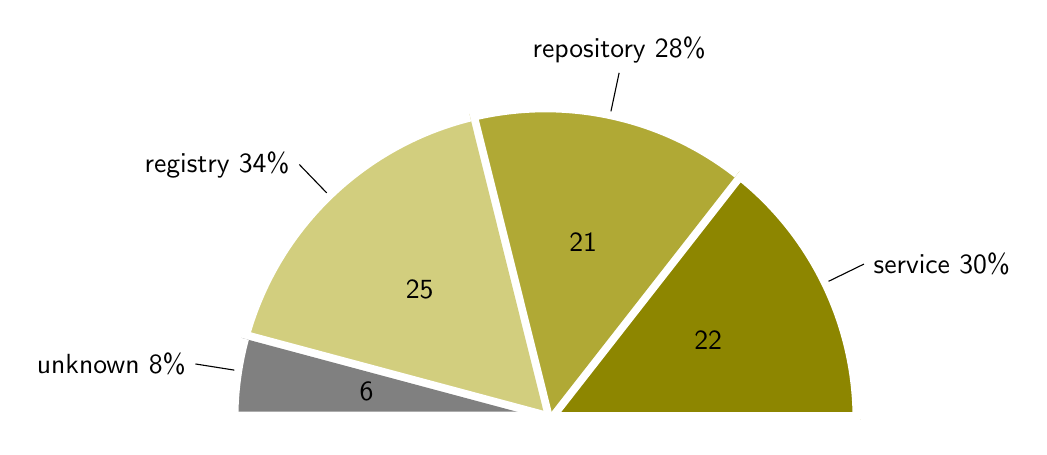
\begin{tikzpicture}
        
%     31 registry
%     21 repository
%     22 service

% TODO: make color more greenish and use same color above
      \foreach \start/\end/\middle/\number/\percent/\color/\anchor/\name in {
		  0/52/26/22/30/olive!100/right/service,
		  52/104/78/21/28/olive!70/above/repository,
		  104/165/134/25/34/olive!40/left/registry,
		  165/180/171/6/8/gray/left/unknown}
	  {
		\draw[fill=\color,draw=white,line width=2mm] (0,0) -- (\end:4cm) arc (\end:\start:4cm)
		  node at (\middle:2.3cm) {\number};
		\draw (\middle:4cm) -- (\middle:4.5cm) node[\anchor] {\name~\percent\%};
	  };        
     \draw[draw=white,line width=2mm] (0:4cm) -- (0,0);

    \end{tikzpicture}
    \end{tikzfigure}

  \end{minipage}%
  \hspace{1em}
  \begin{adjustbox}{valign=t}\begin{minipage}[t]{0.62\linewidth}

      Topic repositories collect terminologies from one subject area.  Around a
      third (25) are topic registries/repositories/services.  The most frequent
      topics are:

      % TODO: bar chart

     \begin{itemize} 
      \item %DDC 610: 
          \textbf{medicine \& health} (9): METeOR, HeTOP, DIMDI\ldots
      \item %DDC 57x: 
          \textbf{biology and life sciences} (7): GFBio, BioPortal, AberOWL\ldots 
      \item %DDC 550 + 910: 
          \textbf{earth sciences and geography} (3): NERC, Marine Metadata, DGIWG
      \item %DDC 4xx: 
          \textbf{language} (2): ISOcat, CLARIN 
      \item %DDC 700: 
          \textbf{arts} (2): KulturNav, museumsvokabular.de 
     \end{itemize}

  \end{minipage}\end{adjustbox}
}

\note[angle=-150,width=205mm,rotate=2,targetoffsetx=-93mm,targetoffsety=-13mm]
{Five have already been closed in the last three years and several have never
been more then a prototype!}

%Persistence?!


%* description and capabilities of terminology registries
%    * disciplines
%    * hosting institution
%    * target audience
%    * terminology management


% references and outlook
\begin{columns}
\column{.6}
\block{References}{
  \vspace{0.5em}
  \begin{center}\mbox{}\vspace{-\baselineskip}
  \printbibliography[heading=none]
  \end{center}
}
\column{.4}
\block{What to do next?}{
  \begin{itemize}
    \renewcommand{\labelitemi}{\color{GBVDark}\textbf{$\rightarrow$}}
    \item Put terminologies into a Terminology Service
	\item Register terminologies/registries in BARTOC
	\item Express terminologies/services with JSKOS
	\item Use existing terminology services
    \item Think about registry persistence
    \item Join RDA Vocabulary Services Interest Group
  \end{itemize}
}
\end{columns}


% end of poster content

\end{document}
